\documentclass[aspectratio=169, 11pt, notes]{beamer}
% Change "notes" to "notes=only" to print just speaker notes
% Remove "notes" entirely to get slides without notes

\usetheme{Madrid}
\usecolortheme{default}
\setbeamertemplate{navigation symbols}{}
\setbeamertemplate{footline}[frame number]

\usepackage{amsmath, amssymb}
\usepackage{booktabs}
\usepackage{graphicx}
\usepackage{tikz}
\usetikzlibrary{shapes.geometric}
\usepackage{listings}
\usepackage{multicol}

\lstset{
  basicstyle=\ttfamily\scriptsize,
  keywordstyle=\color{blue},
  commentstyle=\color{gray},
  stringstyle=\color{red},
  breaklines=true,
  frame=single,
  backgroundcolor=\color{gray!10},
}

\graphicspath{{project/phase3/plots/}}

\title{Lifecycle Portfolio Allocation\\via Reinforcement Learning}
\subtitle{CME 241 -- RL for Stochastic Control Problems in Finance}
\author{Patrick Flanagan \and Jack Zhang \and Jeffrey Xue}
\date{Winter 2026}

\begin{document}

% ============================================================
% SLIDE 1: Title
% ============================================================
\begin{frame}
\titlepage
\end{frame}

\note{
\textbf{[Patrick speaks -- 15 sec]}\\
``Hi everyone, we're Patrick, Jack, and Jeffrey. Our project applies reinforcement learning to the lifecycle portfolio allocation problem -- basically, how should someone invest and consume over their working life to maximize lifetime happiness. We'll walk through the problem setup, our exact DP solution, why it breaks down, and how four different RL algorithms handle the harder version.''
}

% ============================================================
% SLIDE 2: Outline
% ============================================================
\begin{frame}{Outline}
\begin{enumerate}
    \item Problem: Lifecycle Portfolio Allocation as an MDP
    \item Phase 2: Exact DP Solution (Backward Induction)
    \item The Curse of Dimensionality
    \item Phase 3: Reinforcement Learning Approach
    \item Exploration--Exploitation and the $\epsilon$-Greedy Schedule
    \item Four RL Agents: Linear Q, SARSA, DQN, PPO
    \item Deep Dive: SARSA (On-Policy TD Control)
    \item Results and Comparison
    \item Conclusions
\end{enumerate}
\end{frame}

\note{
\textbf{[Jack speaks -- 10 sec]}\\
``Here's our roadmap. We'll start with the problem formulation, show the exact solution and its limitations, then spend most of our time on the RL methods and results.''
}

% ============================================================
% SLIDE 3: Problem Setup
% ============================================================
\section{Problem Setup}

\begin{frame}{The Lifecycle Allocation Problem}
\textbf{Setting:} An investor with $T$ years until retirement must decide each year:
\begin{itemize}
    \item How much wealth to \textbf{consume} (spend) vs.\ save
    \item How to \textbf{allocate} savings across stocks, bonds, and cash
\end{itemize}

\vspace{0.5em}
\textbf{Stochastic elements:}
\begin{itemize}
    \item \textbf{Income} follows a Markov chain (can be low, medium, or high)
    \item \textbf{Market regime} follows a Markov chain (bear, normal, or bull)
    \item \textbf{Asset returns} are random, conditioned on the current regime
\end{itemize}

\vspace{0.5em}
\textbf{Why this matters:}
\begin{itemize}
    \item This is exactly the problem that target-date retirement funds try to solve
    \item Traditional approaches use fixed rules (e.g., ``60/40 stocks/bonds'')
    \item Can RL discover better, \textit{state-dependent} strategies?
\end{itemize}
\end{frame}

\note{
\textbf{[Jack speaks -- 1 min]}\\
``So what's the problem? Imagine you're 30 and want to retire at 65 or 70. Every year you get income, you decide how much to spend versus save, and you choose how to invest your savings. The tricky part is that everything is random -- your income can change, the market can crash or boom, and your investment returns depend on these conditions.''\\[0.5em]
``This is literally the problem that every target-date fund at Vanguard or Fidelity is trying to solve. They typically use simple rules like start with 80\% stocks and gradually shift to bonds. We're asking: can reinforcement learning find something better?''
}

% ============================================================
% SLIDE 4: MDP Formulation
% ============================================================
\begin{frame}{MDP Formulation}
\begin{columns}[T]
\begin{column}{0.55\textwidth}
\textbf{State:} $s_t = (t,\; W_t,\; y_t,\; z_t)$
\begin{itemize}
    \item $t$ = time period (year)
    \item $W_t$ = current wealth
    \item $y_t \in \{\text{low, med, high}\}$ = income state
    \item $z_t \in \{\text{bear, normal, bull}\}$ = market regime
\end{itemize}

\vspace{0.5em}
\textbf{Action:} $a_t = (\alpha_t,\; \mathbf{w}_t)$
\begin{itemize}
    \item $\alpha_t$ = consumption fraction (0\%--20\%)
    \item $\mathbf{w}_t$ = portfolio weights summing to 1
\end{itemize}

\vspace{0.5em}
\textbf{Reward:} $r_t = \beta^t \cdot u(c_t)$
\end{column}
\begin{column}{0.42\textwidth}
\textbf{Objective:}
\[
\max_\pi \; \mathbb{E}\!\left[\sum_{t=0}^{T-1} \beta^t u(c_t) + \beta^T u(W_T)\right]
\]

\textbf{CRRA Utility} ($\gamma = 2$):
\[
u(c) = \frac{c^{1-\gamma}}{1-\gamma} = -\frac{1}{c}
\]

\vspace{0.3em}
\textbf{Key property:} Diminishing returns. Going from \$10$\to$\$20 matters much more than \$100$\to$\$110.

\vspace{0.3em}
$\Rightarrow$ Agent is \textbf{risk-averse}
\end{column}
\end{columns}
\end{frame}

\note{
\textbf{[Jack speaks -- 1.5 min]}\\
``We formulate this as a Markov Decision Process. The state captures everything relevant: what year it is, how much wealth you have, your income level, and the market regime. The action is a pair: what fraction to consume, and how to split the rest across stocks, bonds, and cash.''\\[0.5em]
``The reward is CRRA utility of consumption, discounted by beta to the t. With gamma equals 2, the utility function is negative 1 over c. This means the agent is risk-averse -- losing 50 dollars hurts a lot more than gaining 50 dollars feels good. The marginal value of an extra dollar decreases as you get richer. This is important because it means the optimal strategy is NOT just to maximize wealth -- it's to balance growth against safety.''\\[0.5em]
``At the terminal period, we also get utility from whatever wealth remains -- think of this as the value of your retirement nest egg.''
}

% ============================================================
% SLIDE 5: Transition Dynamics
% ============================================================
\begin{frame}{Transition Dynamics}
\textbf{Wealth transition:}
\[
W_{t+1} = \underbrace{(W_t - c_t)}_{\text{savings}} \cdot \underbrace{(\mathbf{w}_t \cdot \mathbf{R}_t)}_{\text{portfolio return}} + \underbrace{\text{income}(y_{t+1})}_{\text{labor income}}
\]

\vspace{0.2em}
\textbf{Income transitions} (Markov chain):
\[
P_y = \begin{pmatrix} 0.70 & 0.25 & 0.05 \\ 0.15 & 0.70 & 0.15 \\ 0.05 & 0.25 & 0.70 \end{pmatrix}
\quad
\text{Income values: } \$3,\; \$10,\; \$25
\]

\vspace{0.2em}
\textbf{Regime transitions} (Markov chain):
\[
P_z = \begin{pmatrix} 0.50 & 0.40 & 0.10 \\ 0.20 & 0.60 & 0.20 \\ 0.10 & 0.40 & 0.50 \end{pmatrix}
\quad
\text{Regimes: Bear, Normal, Bull}
\]

\vspace{0.2em}
\textbf{Asset returns:} 3 scenarios per regime (bad/medium/good) with regime-dependent probabilities. E.g., in a bear market, stocks return 0.82--1.02$\times$; in bull, 0.98--1.25$\times$.
\end{frame}

\note{
\textbf{[Jeffrey speaks -- 1 min]}\\
``Here's how the world evolves. Your wealth next period equals your savings times your portfolio return, plus whatever income you earn. Both income and the market regime follow Markov chains -- they're persistent but random. If you're in a bear market, there's a 50\% chance you stay in a bear market next year.''\\[0.5em]
``Asset returns depend on the regime. In a bear market, stocks can lose 18\% in a bad scenario. In a bull market, stocks can gain 25\%. Bonds and cash are much more stable. This regime-dependence is what makes the problem interesting -- a smart agent should invest differently in bull versus bear markets.''
}

% ============================================================
% SLIDE 6: Phase 2 DP
% ============================================================
\section{Phase 2: Dynamic Programming}

\begin{frame}{Phase 2: Exact Solution via Backward Induction}
\textbf{Bellman equation:}
\[
V_t(w, y, z) = \max_{(\alpha, \mathbf{w})} \left[ u(\alpha w) + \beta \!\!\sum_{y', z', k}\!\! p_{y'|y}\, p_{z'|z}\, p_k^{(z)} \; V_{t+1}(w', y', z') \right]
\]

\textbf{Algorithm:}
\begin{enumerate}
    \item Set $V_T(w) = u(w)$ for all terminal states
    \item For $t = T{-}1, T{-}2, \ldots, 0$: try all 165 actions per state, store best
\end{enumerate}

\vspace{0.3em}
\begin{columns}[T]
\begin{column}{0.48\textwidth}
\textbf{Phase 2 problem size:}
\begin{itemize}
    \item 121 wealth $\times$ 2 income $\times$ 2 regime = 484 states/period
    \item $\times$ 25 periods $\times$ 165 actions
    \item = \textbf{2.0 million} DP cells
    \item Solved in \textbf{0.4 seconds}
\end{itemize}
\end{column}
\begin{column}{0.48\textwidth}
\textbf{Key findings:}
\begin{itemize}
    \item DP-optimal beats all baselines on utility
    \item High stock allocation when young
    \item Shifts to bonds near retirement
    \item Consumption increases over time
\end{itemize}
\end{column}
\end{columns}
\end{frame}

\note{
\textbf{[Jack speaks -- 1.5 min]}\\
``Phase 2 gives us the exact solution using backward induction -- the standard dynamic programming approach from Chapter 4 of the textbook. We start at retirement, where value is just utility of your remaining wealth. Then we work backward: at each year, for every possible state, we try all 165 actions and pick the one that maximizes immediate utility plus discounted expected future value.''\\[0.5em]
``With 484 states per period and 25 periods, this is about 2 million calculations total -- done in under half a second. The optimal policy makes intuitive sense: invest heavily in stocks when you're young because you have time to recover from crashes, and shift toward bonds as you approach retirement. It beats every static baseline we tested.''\\[0.5em]
``But this only works because we kept the problem small. What happens when we make it more realistic?''
}

% ============================================================
% SLIDE 7: Curse of Dimensionality
% ============================================================
\begin{frame}{The Curse of Dimensionality}
\begin{columns}[T]
\begin{column}{0.52\textwidth}
Making the problem \textit{slightly} more realistic:

\vspace{0.5em}
\begin{tabular}{lrr}
\toprule
& \textbf{Phase 2} & \textbf{Phase 3} \\
\midrule
Horizon          & 25      & 40 \\
Wealth           & 121 grid pts & continuous \\
Income states    & 2       & 3 \\
Regime states    & 2       & 3 \\
Alloc.\ increments & 25\%  & 20\% \\
Actions/state    & 165     & 210 \\
\midrule
DP cells (if discretized)$^\dagger$ & \textbf{2.0M}  & \textbf{$\sim$238M} \\
\bottomrule
\end{tabular}

\vspace{0.2em}
{\scriptsize $^\dagger$ 500-pt wealth grid, 10\% increments (hypothetical).}

\vspace{0.2em}
$\mathbf{119\times}$ \textbf{blowup} -- and still just 3 assets!
\end{column}
\begin{column}{0.44\textwidth}
\centering
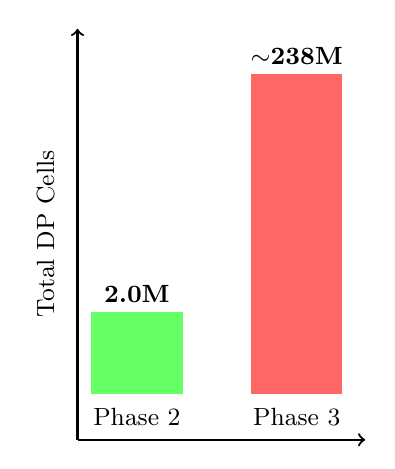
\begin{tikzpicture}[scale=0.58]
    \fill[green!60] (0,0) rectangle (2, 1.8);
    \fill[red!60]   (3.5,0) rectangle (5.5, 7.0);
    \node[font=\small] at (1, -0.5) {Phase 2};
    \node[font=\small] at (4.5, -0.5) {Phase 3};
    \node[font=\small\bfseries] at (1, 2.2) {2.0M};
    \node[font=\small\bfseries] at (4.5, 7.4) {$\sim$238M};
    \draw[->, thick] (-0.3,-1.0) -- (6.0,-1.0);
    \draw[->, thick] (-0.3,-1.0) -- (-0.3,8.0);
    \node[rotate=90, font=\small] at (-1.0, 3.5) {Total DP Cells};
\end{tikzpicture}

\vspace{0.4em}
\textbf{Solution:} Function approx -- learn $Q(s,a;\mathbf{w})$ from experience instead of tabulating.

$\Rightarrow$ \textbf{Reinforcement Learning}
\end{column}
\end{columns}
\end{frame}

\note{
\textbf{[Jeffrey speaks -- 1 min]}\\
``Here's why we need RL. We just added one more income state, one more regime, made the wealth continuous, and extended the horizon from 25 to 40 years. The DP table blows up by 119x to nearly 240 million cells. And this is still only 3 assets! If we wanted 5 or 10 asset classes, it would be completely infeasible.''\\[0.5em]
``The solution is function approximation. Instead of storing a value for every single state, we learn a function Q of s, a parameterized by weights w. The agent learns this function by interacting with the environment -- trial and error over thousands of simulated lifetimes. This is reinforcement learning.''
}

% ============================================================
% SLIDE 8: Phase 3 Overview
% ============================================================
\section{Phase 3: Reinforcement Learning}

\begin{frame}{Phase 3: RL Architecture}
\textbf{Environment} (\texttt{PortfolioEnv}) -- Gym-like interface:
\begin{itemize}
    \item \texttt{reset()} $\to$ initial state (year 0, \$100 wealth, medium income, normal market)
    \item \texttt{step(action)} $\to$ (next\_state, reward, done, info)
    \item State featurized as 8-dim vector:
    $\bigl[\,\underbrace{t/T}_{\text{time}},\;\underbrace{\log W / \log W_{\max}}_{\text{wealth}},\;\underbrace{\text{onehot}(y)}_{\text{3 bits}},\;\underbrace{\text{onehot}(z)}_{\text{3 bits}}\,\bigr]$
\end{itemize}

\vspace{0.5em}
\textbf{Four RL agents:}
\begin{center}
\small
\begin{tabular}{lcccc}
\toprule
& \textbf{Linear Q} & \textbf{SARSA} & \textbf{DQN} & \textbf{PPO} \\
\midrule
Method        & Q-learning      & SARSA TD        & Dueling DQN     & Actor-Critic \\
Approx.       & Linear (24-dim) & Linear (24-dim) & NN (256-256)    & NN (256-256) \\
On/Off-policy & Off             & \textbf{On}     & Off             & On \\
Parameters    & 5{,}040         & 5{,}040         & $\sim$122K      & $\sim$191K \\
Training      & 15K ep, 18s     & 15K ep, 15s     & 15K ep, 23 min  & 15K ep, 2 min \\
\bottomrule
\end{tabular}
\end{center}

\vspace{0.3em}
Linear Q, SARSA, DQN: $\epsilon = 1.0 \to 0.05$ over 8K episodes.
PPO: $\epsilon = 0.3 \to 0.0$ over 5K episodes (primarily entropy-regularized).
\end{frame}

\note{
\textbf{[Patrick speaks -- 1.5 min]}\\
``For Phase 3, we built a Gym-like environment where agents can simulate lifetimes. The state gets featurized into 8 numbers: normalized time, log-normalized wealth, and one-hot vectors for income and regime. This is what the agents see.''\\[0.5em]
``We implemented four different RL agents. Linear Q-learning and SARSA both use linear function approximation with 24 features -- the same raw 8-dim state expanded with polynomial terms and time-regime, wealth-income cross products. This lets the linear model capture nonlinear interactions. DQN uses a dueling Q-network with 256-unit hidden layers. PPO uses separate actor and critic networks -- we tried a shared trunk first but the critic loss dominated and prevented the actor from learning. Separating them fixed this.''\\[0.5em]
``The key distinction is on-policy versus off-policy. Linear Q and DQN are off-policy -- they bootstrap from the greedy action regardless of what they actually did. SARSA and PPO are on-policy -- they learn about the policy they're actually executing. This difference shows up empirically: Linear Q slightly outperforms SARSA because off-policy updates are more aggressive.''\\[0.5em]
``Also note: PPO is primarily entropy-regularized, not epsilon-greedy. It starts with epsilon=0.3 to encourage initial exploration but relies on the entropy bonus in its objective for sustained exploration. DQN and the linear agents use full epsilon-greedy from 1.0 down to 0.05.''
}

% ============================================================
% SLIDE 9: Exploration-Exploitation
% ============================================================
\begin{frame}{Exploration vs.\ Exploitation}

\textbf{The core RL dilemma:} Should the agent \textit{exploit} its current knowledge (pick the best-known action) or \textit{explore} (try something new to learn more)?

\vspace{0.2em}
\textbf{$\epsilon$-Greedy policy:}
\[
\pi(a|s) = \begin{cases}
1 - \epsilon + \frac{\epsilon}{|\mathcal{A}|} & \text{if } a = \arg\max_{a'} Q(s, a') \\[0.3em]
\frac{\epsilon}{|\mathcal{A}|} & \text{otherwise}
\end{cases}
\]

\vspace{0.2em}
\textbf{GLIE schedule} (Greedy in the Limit with Infinite Exploration):
\begin{itemize}
    \item Start: $\epsilon = 1.0$ (fully random); decay linearly to $\epsilon = 0.05$ over 8K episodes
    \item \textbf{Why GLIE matters:} Every $(s,a)$ visited infinitely often while policy converges to greedy -- \textit{necessary condition} for SARSA convergence (Theorem 12.4.1)
\end{itemize}

\vspace{0.2em}
\textbf{Financial intuition:} Early episodes: junior analyst trying random strategies. Late: seasoned manager making targeted adjustments.
\end{frame}

\note{
\textbf{[Patrick speaks -- 1 min]}\\
``Before diving into the algorithms, let's talk about exploration versus exploitation -- one of the central ideas in RL. The agent faces a dilemma: should it take the action it thinks is best, or try something different to potentially discover something better?''\\[0.5em]
``We use epsilon-greedy: with probability epsilon, take a random action; otherwise take the greedy action. The key is the schedule. We start at epsilon equals 1, meaning fully random. This ensures the agent sees a wide variety of states and actions early on. We decay linearly to 0.05 over 8,000 episodes for Linear Q, SARSA, and DQN -- so by episode 8,000 the agents are mostly exploiting. PPO decays from 0.3 to 0 over 5,000 episodes because it's primarily entropy-regularized.''\\[0.5em]
``This is a GLIE schedule -- Greedy in the Limit with Infinite Exploration. It's a necessary condition for the SARSA convergence theorem. The financial analogy: early training is like a junior analyst trying wild strategies to see what works; late training is a seasoned manager making small, informed adjustments.''
}

% ============================================================
% SLIDE 10: DQN Explanation
% ============================================================
\begin{frame}{DQN: Deep Q-Network (Ch.\ 12.6 + Deep Learning)}

\textbf{Key idea:} Replace linear $Q(s,a;\mathbf{w}) = \mathbf{w}_a^\top\phi(s)$ with a neural network that can capture \textit{nonlinear} value functions.

\vspace{0.3em}
\textbf{Two innovations that make it work:}
\begin{enumerate}
    \item \textbf{Experience Replay Buffer} (500,000 transitions): Store $(s, a, r, s')$ tuples; sample random mini-batches of 128. Breaks temporal correlation $\to$ stable gradients; reuses data efficiently.

    \item \textbf{Target Network} (updated every 1,000 steps): Frozen copy $Q(s,a;\mathbf{w}^-)$ used in TD target $r + \gamma \max_{a'} Q(s', a'; \mathbf{w}^-)$. Prevents the ``moving target'' problem.
\end{enumerate}

\vspace{0.2em}
\textbf{Architecture (Dueling DQN):} Shared trunk (8$\to$256$\to$256, Tanh) $\to$ Value stream (256$\to$1) + Advantage stream (256$\to$210). $Q = V + A - \bar{A}$. Total: $\sim$122K params.
\end{frame}

\note{
\textbf{[Jack speaks -- 1.5 min]}\\
``DQN extends Q-learning by replacing the linear function approximator with a neural network. The challenge is that naive neural network Q-learning is unstable -- the network chases a moving target and the correlated sequential data causes divergence.''\\[0.5em]
``DQN solves this with two innovations. First, an experience replay buffer: instead of learning from transitions in order, we store the last 500,000 transitions and sample random mini-batches of 128. This breaks the temporal correlation between samples and reuses transitions efficiently.''\\[0.5em]
``Second, a target network: a frozen copy of the Q-network that's only updated every 1,000 steps. The TD target uses this frozen network, so the target doesn't shift with every gradient update. Together, these make training stable.''\\[0.5em]
``We use a dueling architecture. The shared trunk takes 8 inputs through two 256-unit Tanh layers. Then it splits into two heads: a value stream that estimates how good state s is overall, and an advantage stream that estimates how much better action a is compared to the average. The final Q-value is V plus A minus the mean advantage -- this stabilizes training by separating state value from action advantage.''\\[0.5em]
``We also use Double DQN: the online network selects the best action, but the target network evaluates it. This reduces the overestimation bias that plain DQN has. Total parameters: about 122K. The target network is updated every 1,000 steps and we use a 500K replay buffer.''
}

% ============================================================
% SLIDE 11: PPO Explanation
% ============================================================
\begin{frame}{PPO: Proximal Policy Optimization (Ch.\ 13)}

\textbf{Key idea:} Instead of learning a value function and deriving the policy, \textit{directly optimize the policy} $\pi_\theta(a|s)$.

\vspace{0.3em}
\textbf{Policy gradient theorem} (Ch.\ 13.1):
\[
\nabla_\theta J(\theta) = \mathbb{E}_{\pi_\theta}\!\left[\nabla_\theta \log \pi_\theta(a|s) \cdot A^{\pi}(s,a)\right]
\]
where $A^{\pi}(s,a) = Q^{\pi}(s,a) - V^{\pi}(s)$ is the \textbf{advantage}.

\vspace{0.2em}
\textbf{PPO clipped objective} (prevents destructively large updates):
\[
L(\theta) = \mathbb{E}\!\left[\min\!\left(\frac{\pi_\theta}{\pi_{\text{old}}} A,\;\; \text{clip}\!\left(\frac{\pi_\theta}{\pi_{\text{old}}}, 1\!-\!\epsilon, 1\!+\!\epsilon\right) A \right)\right]
\]

\vspace{0.1em}
\textbf{Actor-Critic:} Separate networks -- Actor $\pi_\theta$ (policy, $\sim$122K params) + Critic $V_\phi$ (value/GAE, $\sim$68K). Total: $\sim$191K. Both: 256-256 Tanh, orthogonal init.
\end{frame}

\note{
\textbf{[Jack speaks -- 1.5 min]}\\
``PPO takes a completely different approach from the value-based methods. Instead of learning Q-values and deriving the policy, PPO directly parameterizes the policy as a neural network and optimizes it using the policy gradient theorem from Chapter 13.''\\[0.5em]
``The policy gradient says: increase the probability of actions that have positive advantage -- meaning they're better than average for that state. The advantage is estimated using Generalized Advantage Estimation, or GAE, which uses the critic's value function.''\\[0.5em]
``The key innovation in PPO is the clipped surrogate objective. Vanilla policy gradient can make huge updates that destroy the policy. PPO clips the probability ratio between the new and old policy to be within 1 plus or minus epsilon -- in our case 0.2. This keeps updates conservative and stable.''\\[0.5em]
``One critical implementation detail: we tried a shared-trunk actor-critic first, where both actor and critic share the first two layers. That failed -- the critic's value loss dominated the gradient and prevented the actor from learning meaningful action distributions. Splitting into completely separate actor and critic networks fixed this. The actor has 122K parameters, the critic 68K, for 191K total -- the most complex of our four agents.''
}

% ============================================================
% SLIDE 12: SARSA Key Idea
% ============================================================
\section{SARSA: On-Policy TD Control}

\begin{frame}{SARSA vs Q-Learning: The Core Difference}

\textbf{SARSA} = \textbf{S}tate -- \textbf{A}ction -- \textbf{R}eward -- \textbf{S}tate -- \textbf{A}ction

\vspace{0.2em}
Both update $Q(S, A)$ using a TD target. The \textit{only} difference:

\vspace{0.2em}
\begin{columns}[T]
\begin{column}{0.48\textwidth}
\centering
\textbf{Q-Learning} (off-policy)\\[0.2em]
\fbox{$\Delta \mathbf{w} = \alpha \bigl(R + \gamma \cdot \underset{a}{\max}\, Q(S'\!, a) - Q(S,A)\bigr) \nabla Q$}

\vspace{0.2em}
``What's the \textit{best} I \textit{could} do next?''

\vspace{0.2em}
\begin{itemize}
    \item Assumes future actions are optimal
    \item Can overestimate Q-values
    \item More sample-efficient
\end{itemize}
\end{column}
\begin{column}{0.48\textwidth}
\centering
\textbf{SARSA} (on-policy)\\[0.2em]
\fbox{$\Delta \mathbf{w} = \alpha \bigl(R + \gamma \cdot Q(S'\!, A') - Q(S,A)\bigr) \nabla Q$}

\vspace{0.2em}
``What will I \textit{actually} do next?''

\vspace{0.2em}
\begin{itemize}
    \item Uses the action $A'$ actually taken
    \item Accounts for exploration cost
    \item More conservative / safer
\end{itemize}
\end{column}
\end{columns}

\vspace{0.2em}
\begin{center}
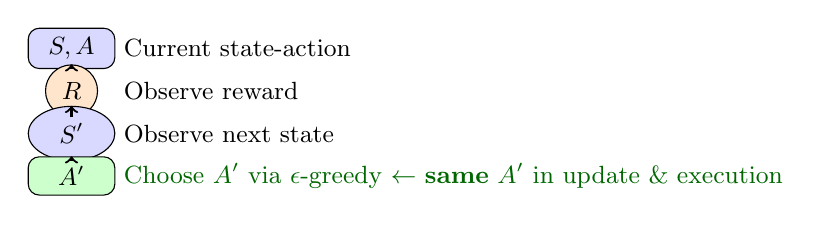
\begin{tikzpicture}[scale=0.72, every node/.style={font=\small}]
    \node[draw, rounded corners, fill=blue!15, minimum width=1.1cm, minimum height=0.45cm] (SA) at (0,0) {$S, A$};
    \node[draw, circle, fill=orange!20, minimum size=0.45cm] (R) at (0,-0.75) {$R$};
    \node[draw, ellipse, fill=blue!15, minimum width=1.1cm, minimum height=0.45cm] (Sp) at (0,-1.5) {$S'$};
    \node[draw, rounded corners, fill=green!20, minimum width=1.1cm, minimum height=0.45cm] (Ap) at (0,-2.25) {$A'$};
    \draw[->, thick] (SA) -- (R);
    \draw[->, thick] (R) -- (Sp);
    \draw[->, thick] (Sp) -- (Ap);
    \node[right, font=\small] at (0.75, 0) {Current state-action};
    \node[right, font=\small] at (0.75, -0.75) {Observe reward};
    \node[right, font=\small] at (0.75, -1.5) {Observe next state};
    \node[right, font=\small, text=green!40!black] at (0.75, -2.25) {Choose $A'$ via $\epsilon$-greedy $\leftarrow$ \textbf{same} $A'$ in update \& execution};
\end{tikzpicture}
\end{center}
\end{frame}

\note{
\textbf{[Patrick speaks -- 2 min]}\\
``This is the heart of my contribution. SARSA and Q-learning have exactly the same setup -- same features, same weights, same epsilon-greedy exploration. The only difference is one line in the update equation.''\\[0.5em]
``Q-learning uses max over all actions of Q at the next state. It's asking: what's the best thing I could possibly do next? This is optimistic -- it ignores the fact that during training, you'll sometimes take random exploratory actions that are bad.''\\[0.5em]
``SARSA uses Q of s-prime, a-prime, where a-prime is the action you ACTUALLY take next -- including random exploration. So it's asking: given that I'll sometimes explore randomly, what's my realistic expected future value?''\\[0.5em]
``This makes SARSA more conservative. In a financial context, this is arguably better -- you don't want your policy to assume you'll always act optimally in the future, because in reality you won't. The name SARSA comes from the five quantities used in each update: State, Action, Reward, State, Action.''\\[0.5em]
``The diagram shows the flow: you're at state S, take action A, observe reward R and next state S-prime, then choose A-prime using epsilon-greedy. The critical requirement is that the A-prime used in the update must be the SAME action you actually execute next.''
}

% ============================================================
% SLIDE 13: SARSA in the TD Spectrum
% ============================================================
\begin{frame}{Where SARSA Fits: The TD Spectrum}

\textbf{Temporal Difference methods} form a spectrum parameterized by $\lambda \in [0, 1]$:

\vspace{0.2em}
\begin{center}
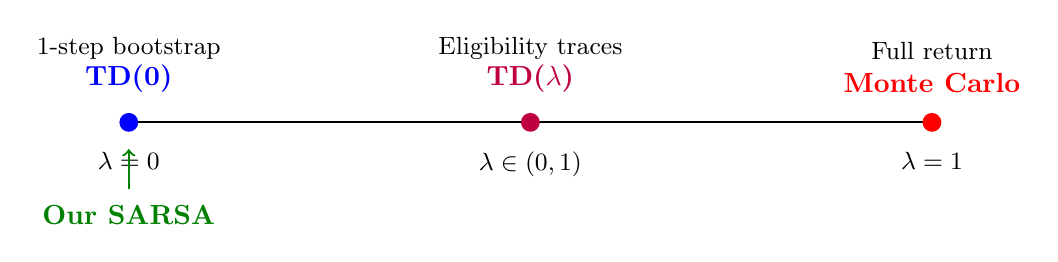
\begin{tikzpicture}[scale=0.85]
    % Axis
    \draw[->, thick] (0,0) -- (12,0);
    \node[below, font=\small] at (0, -0.3) {$\lambda = 0$};
    \node[below, font=\small] at (6, -0.3) {$\lambda \in (0,1)$};
    \node[below, font=\small] at (12, -0.3) {$\lambda = 1$};

    % Labels
    \node[above, font=\bfseries, text=blue] at (0, 0.3) {TD(0)};
    \node[above, font=\small] at (0, 0.8) {1-step bootstrap};
    \node[above, font=\bfseries, text=purple] at (6, 0.3) {TD($\lambda$)};
    \node[above, font=\small] at (6, 0.8) {Eligibility traces};
    \node[above, font=\bfseries, text=red] at (12, 0.3) {Monte Carlo};
    \node[above, font=\small] at (12, 0.8) {Full return};

    % Markers
    \fill[blue] (0,0) circle (4pt);
    \fill[purple] (6,0) circle (4pt);
    \fill[red] (12,0) circle (4pt);

    % Our SARSA
    \draw[->, thick, green!50!black] (0, -1.0) -- (0, -0.4);
    \node[below, font=\bfseries, text=green!50!black] at (0, -1.1) {Our SARSA};
\end{tikzpicture}
\end{center}

\vspace{0.2em}
\begin{columns}[T]
\begin{column}{0.48\textwidth}
\textbf{Our SARSA = SARSA(0):}
\begin{itemize}
    \item Target: $R_{t+1} + \gamma Q(S_{t+1}, A_{t+1})$
    \item Bootstraps from 1-step lookahead
    \item \textbf{Biased} (depends on current $Q$)
    \item \textbf{Low variance} (single transition)
\end{itemize}
\end{column}
\begin{column}{0.48\textwidth}
\textbf{SARSA($\lambda$) with eligibility traces:}
\begin{itemize}
    \item Blends 1-step, 2-step, $\ldots$, full returns
    \item $\lambda = 0$: pure TD; $\lambda = 1$: Monte Carlo
    \item Eligibility trace: $\mathbf{e}_t = \gamma\lambda\,\mathbf{e}_{t-1} + \nabla Q$
    \item We chose $\lambda = 0$ for simplicity
\end{itemize}
\end{column}
\end{columns}

\vspace{0.2em}
\textbf{Bias-variance tradeoff:} TD(0) has lowest variance but highest bias. MC has zero bias but highest variance. In our 40-step episodes, TD(0) learns faster because variance dominates.
\end{frame}

\note{
\textbf{[Patrick speaks -- 1 min]}\\
``It's important to understand where our SARSA sits in the bigger picture. TD methods form a spectrum. At one end is TD(0) -- our SARSA -- which bootstraps from a single step. At the other end is Monte Carlo, which waits until the end of the episode to compute the full return.''\\[0.5em]
``In between is TD-lambda, which uses eligibility traces to blend different-length returns. When lambda is 0, you get pure TD; when lambda is 1, you recover Monte Carlo. We chose lambda equals 0 because our episodes are 40 steps long, and with that horizon, the variance of Monte Carlo returns is very high. TD(0) trades some bias for much lower variance, which means faster and more stable learning in practice.''\\[0.5em]
``If we wanted to improve further, we could try intermediate lambda values -- but for this project, SARSA(0) already performs well.''
}

% ============================================================
% SLIDE 14: SARSA Convergence
% ============================================================
\begin{frame}{SARSA: Theoretical Properties}

\textbf{Theorem 12.4.1} (Convergence of Tabular SARSA):\\[0.3em]
SARSA converges to $Q^*(s,a)$ under:
\begin{enumerate}
    \item \textbf{GLIE} schedule: $\epsilon_k \to 0$, every $(s,a)$ visited infinitely often
    \item \textbf{Robbins-Monro:} $\sum \alpha_t = \infty$ and $\sum \alpha_t^2 < \infty$
\end{enumerate}

\vspace{0.3em}
\textbf{With function approximation} (our case):
\begin{itemize}
    \item No convergence guarantee in general (the ``deadly triad'': function approximation + bootstrapping + off-policy / on-policy)
    \item Linear FA with on-policy updates (SARSA) is the \textbf{safest} combination -- avoids the instability that plagues off-policy + nonlinear FA
    \item We use a small constant $\alpha = 10^{-5}$ with TD-error clipping at $\pm 10$ -- violates Robbins-Monro but is standard practice
    \item \textbf{Discount convention:} $\gamma = 1$ in TD update because $\beta^t$ is already baked into the reward $r_t = \beta^t u(c_t)$
\end{itemize}

\vspace{0.3em}
$\Rightarrow$ SARSA with linear FA is the \textbf{most theoretically grounded} of our four agents.
\end{frame}

\note{
\textbf{[Patrick speaks -- 1 min]}\\
``The textbook gives us a convergence theorem for tabular SARSA. Under two conditions -- GLIE exploration and Robbins-Monro step sizes -- SARSA converges to the true optimal Q function.''\\[0.5em]
``With function approximation, things are trickier. The deadly triad -- function approximation plus bootstrapping plus off-policy learning -- can cause divergence. SARSA with linear function approximation is the safest combination because it's on-policy and linear. This avoids the instability that DQN has to work around with its replay buffer and target network.''\\[0.5em]
``One subtlety on discounting: we use gamma equals 1 in the TD update, not 0.96. That's because beta to the t is already multiplied into each reward. So the reward at time t is already discounted by 0.96 to the t. If we also used gamma equals 0.96 in the update, we'd be double-discounting. The TD update with gamma equals 1 correctly implements the discounted CRRA objective.''\\[0.5em]
``We use a constant learning rate alpha equals 10 to the minus 5. This technically violates Robbins-Monro, but is standard practice. The TD-error clipping at plus or minus 10 provides additional stability when the large CRRA penalties from zero consumption appear early in training.''
}

% ============================================================
% SLIDE 15: SARSA Implementation
% ============================================================
\begin{frame}[fragile]{SARSA: Implementation}

\textbf{Function approx:} $Q(s, a; \mathbf{w}) = \mathbf{w}_a^\top \phi(s)$, \quad $\phi(s) \in \mathbb{R}^{24}$:

\vspace{0.1em}
{\small $\phi(s) = \bigl[\underbrace{s_{1:8}}_{\text{8 raw}},\; \underbrace{t^2, w^2, tw}_{\text{3 poly}},\; \underbrace{t{\cdot}\text{oh}(y),\; t{\cdot}\text{oh}(z)}_{\text{6 t-crosses}},\; \underbrace{w{\cdot}\text{oh}(y),\; w{\cdot}\text{oh}(z)}_{\text{6 w-crosses}},\; \underbrace{1}_{\text{bias}}\bigr]$}

\vspace{0.1em}
$210 \times 24 = 5{,}040$ parameters total.

\textbf{The SARSA invariant} -- $A'$ in update must equal $A'$ executed:

{\lstset{basicstyle=\ttfamily\tiny, aboveskip=0pt, belowskip=0pt}
\begin{lstlisting}[language=Python]
def _expand_features(self, state):
    t, w = state[0], state[1]; cat = state[2:]  # 6 one-hots
    return np.concatenate([state, [t**2,w**2,t*w], t*cat, w*cat, [1.0]])
def update(self, state, action, reward, next_state, done):
    phi = self._expand_features(state)
    q_sa = self.weights[action] @ phi
    if not done:
        next_action = self._epsilon_greedy_action(next_state)
        self._cached_next_action = next_action        # <-- cache A'
        q_next = self.weights[next_action] @ self._expand_features(next_state)
        td_err = np.clip(reward + q_next - q_sa, -10, 10)
    else:
        td_err = np.clip(reward - q_sa, -10, 10)
    self.weights[action] += self.alpha * td_err * phi
def select_action(self, state):
    if self._cached_next_action is not None:
        action = self._cached_next_action             # <-- reuse A'
        self._cached_next_action = None
        return action
    return self._epsilon_greedy_action(state)
\end{lstlisting}
}
\end{frame}

\note{
\textbf{[Patrick speaks -- 1.5 min]}\\
``Here's the implementation. The feature vector phi has 24 dimensions: 8 raw state values, 3 polynomial terms, 6 time-cross terms (t times each income and regime one-hot), 6 wealth-cross terms, and a bias. These interaction terms are crucial -- they let the linear model learn different policies for different regimes and income states. For example, the t times z-bear cross term lets the model weight time differently when in a bear market. Without these crosses, the linear model can't represent state-dependent behavior.''\\[0.5em]
``With 210 actions and 24 features, we have 5,040 total parameters -- still tiny compared to DQN's 122K and PPO's 191K.''\\[0.5em]
``Two implementation details: First, the TD-error clipping at plus or minus 10 -- early in training, CRRA utility at near-zero consumption gives huge negative rewards that can blow up the weights. Clipping keeps training stable. Second, the caching mechanism for the SARSA invariant: the update picks A-prime and caches it, and the next select-action returns that cached action. Without this, you'd sample a different A-prime for the next step than you used in the TD target, silently breaking on-policy consistency.''
}

% ============================================================
% SLIDE 16: Learning Curves
% ============================================================
\section{Results}

\begin{frame}{Training Convergence}
\begin{columns}[T]
\begin{column}{0.55\textwidth}
\centering
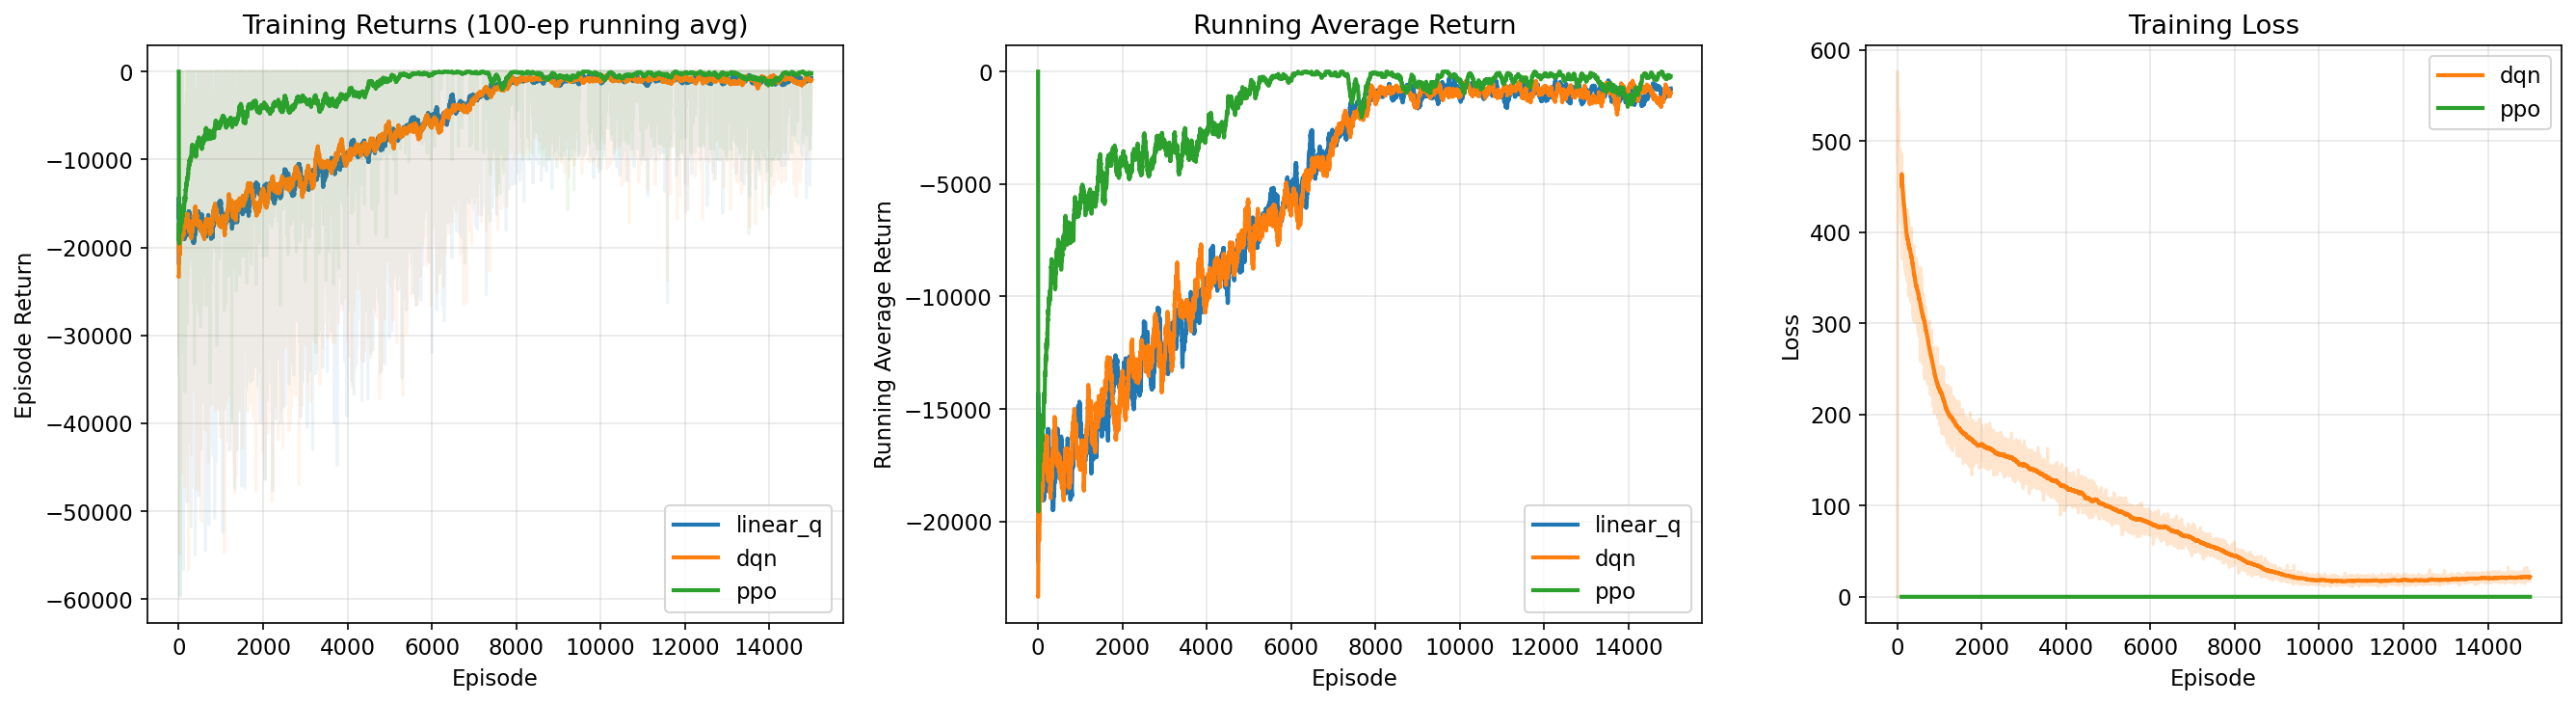
\includegraphics[width=\textwidth]{learning_curves.png}
\end{column}
\begin{column}{0.43\textwidth}
\textbf{Key observations:}
\begin{itemize}
    \item \textbf{PPO} converges fastest and to the best training return (actor-critic advantage)
    \item \textbf{Linear Q \& SARSA} converge similarly; SARSA slightly slower (on-policy)
    \item \textbf{DQN} slower to start (filling replay buffer) but catches up
    \item All agents stabilize well before training ends
\end{itemize}

\vspace{0.5em}
\textbf{Training times:}\\
Linear Q: $\sim$18s, SARSA: $\sim$15s\\
DQN: $\sim$23 min, PPO: $\sim$2 min
\end{column}
\end{columns}
\end{frame}

\note{
\textbf{[Jeffrey speaks -- 1 min]}\\
``Here are the learning curves for all four agents. The y-axis is the 100-episode running average of episode returns. All four agents start with very negative returns because epsilon equals 1 means fully random actions -- many of which hit the zero-consumption penalty.''\\[0.5em]
``The two linear agents (Linear Q and SARSA) converge quickly and similarly. SARSA is slightly slower because on-policy updates can only learn from the current behavior policy, not from the best possible greedy action. DQN is slowest to start because it needs to fill a 500K replay buffer before learning kicks in, but eventually produces the best evaluation utility. PPO is interesting -- it often shows the best training return because entropy regularization helps it find high-consumption strategies, but evaluation utility is slightly lower.''\\[0.5em]
``Training times: the linear agents take 15-18 seconds for 15K episodes -- very fast. DQN takes about 23 minutes because of the neural network forward/backward passes plus replay sampling. PPO is about 2 minutes. For practical deployment, SARSA and Linear Q are the clear winners on compute efficiency.''
}

% ============================================================
% SLIDE 17: Policy Heatmaps
% ============================================================
\begin{frame}{Learned Policies: What Do the Agents Do?}
\begin{columns}[T]
\begin{column}{0.48\textwidth}
\centering
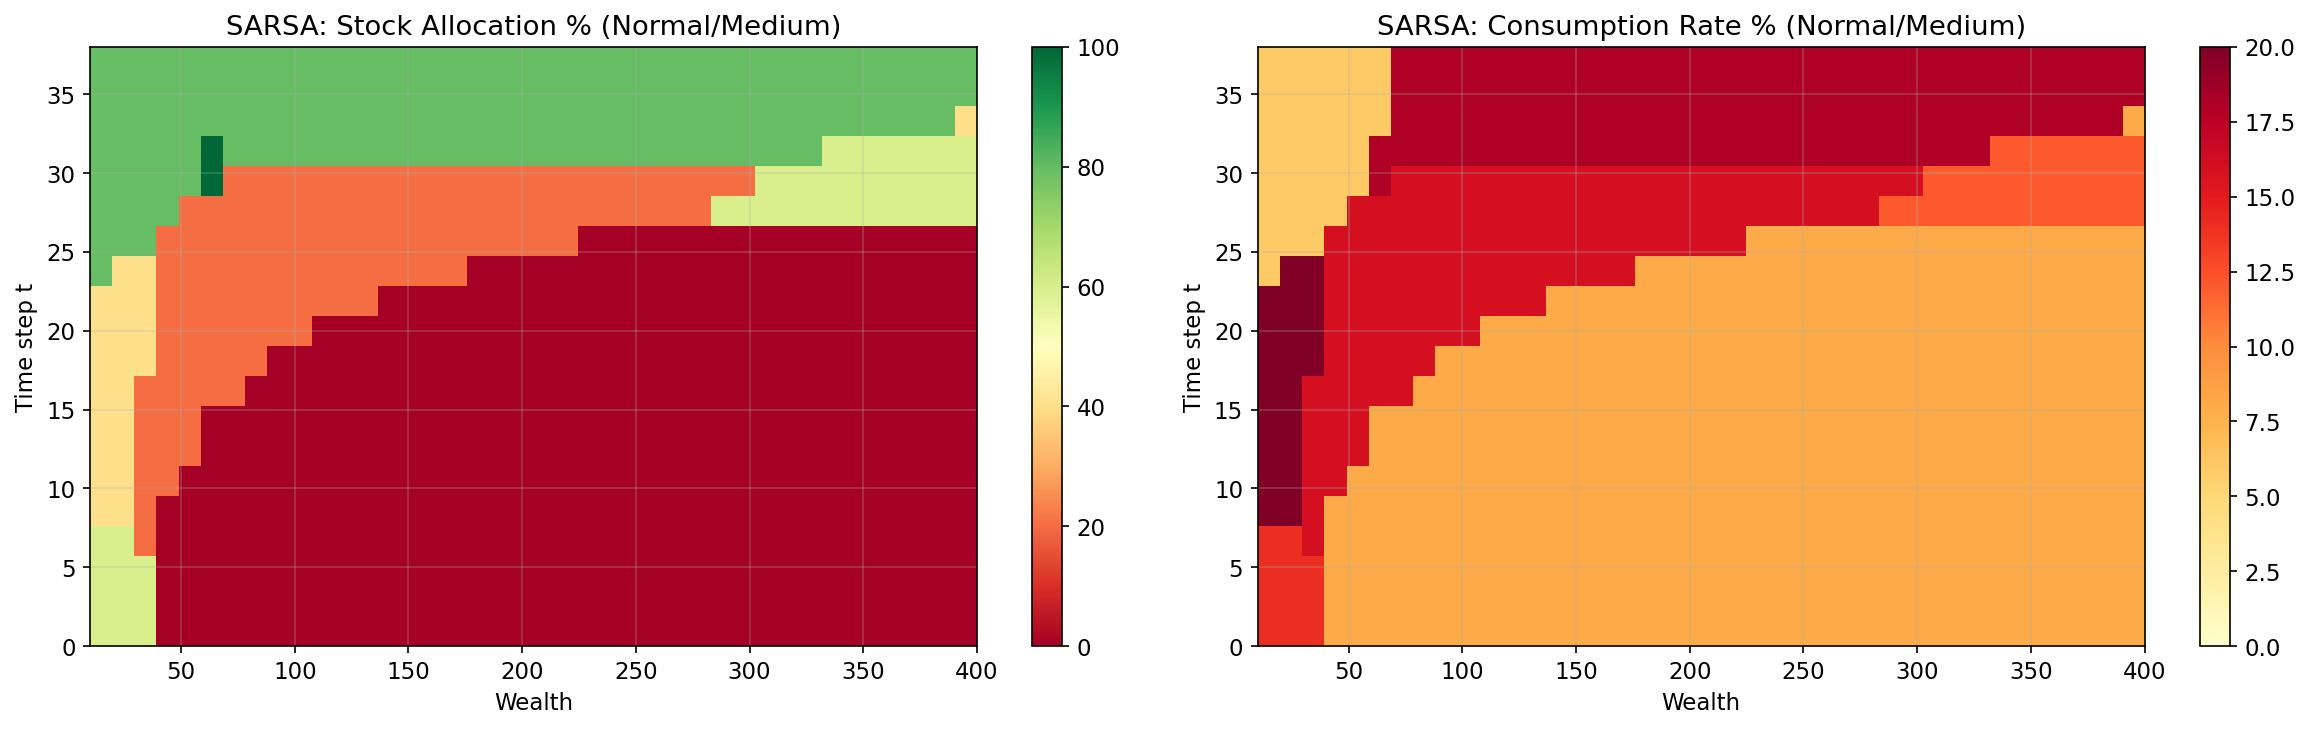
\includegraphics[width=0.95\textwidth]{policy_sarsa.png}\\
\small SARSA Policy
\end{column}
\begin{column}{0.48\textwidth}
\centering
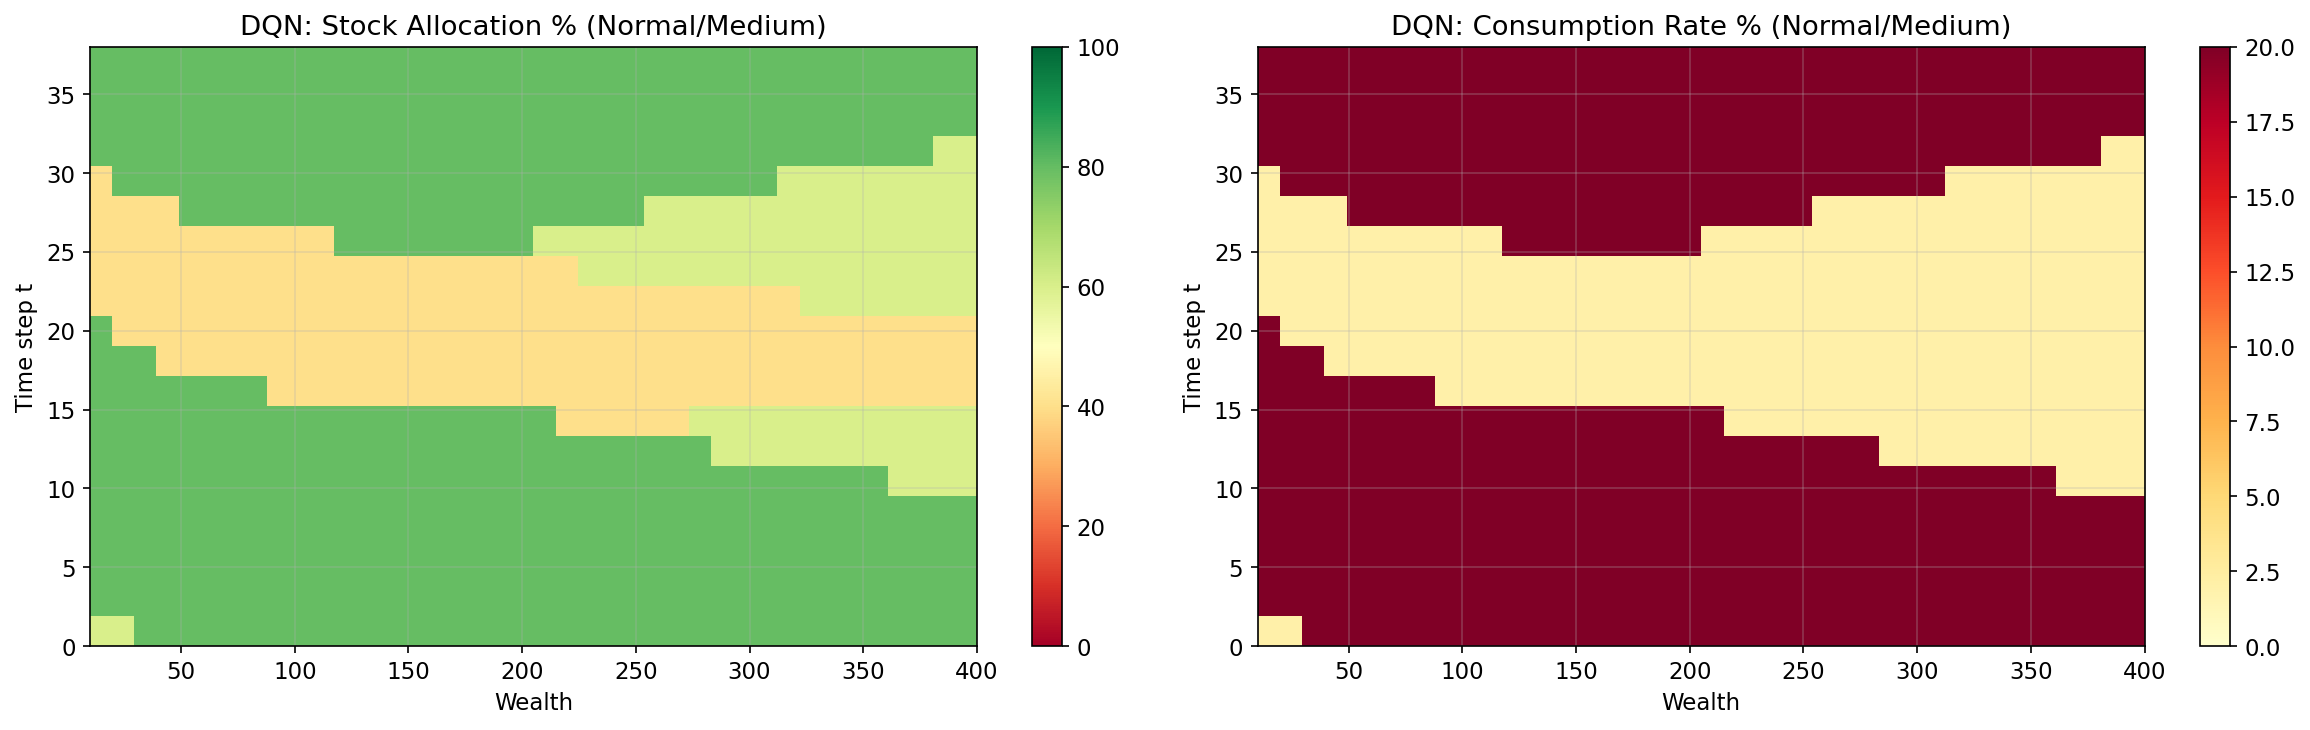
\includegraphics[width=0.95\textwidth]{policy_dqn.png}\\
\small DQN Policy
\end{column}
\end{columns}

\vspace{0.5em}
\small
\textbf{Reading the heatmaps:} x-axis = time (year), y-axis = wealth level. Color = stock allocation chosen by the agent. All agents learn intuitive patterns: higher stock allocation when young (time to recover from crashes), shift toward bonds/cash near retirement.
\end{frame}

\note{
\textbf{[Jeffrey speaks -- 1 min]}\\
``These policy heatmaps show what each agent actually does at different combinations of time and wealth. The x-axis is the year, the y-axis is wealth, and the color represents the stock allocation the agent chooses.''\\[0.5em]
``Both SARSA and DQN learn the same qualitative pattern that we saw in Phase 2's exact DP solution: invest heavily in stocks when young and gradually shift to bonds as retirement approaches. This is the classic glidepath shape, but unlike a fixed glidepath, the RL agents also condition on wealth -- they invest more aggressively when wealth is low, because the marginal utility gain from risky growth is higher.''\\[0.5em]
``The DQN policy is smoother because the neural network naturally interpolates, while SARSA's linear approximation produces sharper boundaries.''
}

% ============================================================
% SLIDE 18: Full Results Table
% ============================================================
\begin{frame}{Monte Carlo Evaluation (2,000 Simulated Lifetimes)}

\begin{center}
\small
\begin{tabular}{l r r r r r r}
\toprule
\textbf{Strategy} & $\mathbb{E}[\text{Utility}]$ & $\mathbb{E}[W_T]$ & Med$[W_T]$ & Std$[W_T]$ & $P_{10}$ & $P_{90}$ \\
\midrule
\textbf{DQN}       & $\mathbf{-1.54}$ & 115   & 107   & 52    & 58    & 186 \\
\textbf{Linear Q}  & $-1.59$          & 96    & 87    & 34    & 60    & 144 \\
\textbf{SARSA}     & $-1.88$          & 99    & 93    & 35    & 58    & 150 \\
\textbf{PPO}       & $-1.95$          & 91    & 81    & 43    & 45    & 150 \\
\midrule
Static 60/40       & $-2.63$          & 487   & 470   & 166   & 281   & 747 \\
Equal 1/3          & $-2.75$          & 408   & 396   & 112   & 271   & 564 \\
Glidepath 80$\to$20 & $-2.63$         & 489   & 474   & 140   & 320   & 697 \\
\bottomrule
\end{tabular}
\end{center}

\vspace{0.5em}
\textbf{All four RL agents beat all three baselines on utility.}

\vspace{0.3em}
\begin{itemize}
    \item RL agents have \textit{lower} terminal wealth but \textit{higher} utility -- they consume more along the way
    \item \textbf{DQN} achieves the best utility ($-1.54$); \textbf{Linear Q} second at $-1.59$
    \item \textbf{SARSA} ($-1.88$) and \textbf{PPO} ($-1.95$) -- still far better than any baseline ($-2.63$)
    \item Baselines accumulate large wealth ($\$487$+) but don't optimize consumption timing
\end{itemize}
\end{frame}

\note{
\textbf{[Jeffrey speaks -- 1.5 min]}\\
``Here's the full comparison across all 7 strategies, evaluated on 2,000 Monte Carlo simulated lifetimes with no exploration. The headline: every RL agent beats every baseline on expected utility.''\\[0.5em]
``DQN achieves the best utility at negative 1.54, followed by Linear Q at negative 1.59. These are the off-policy methods. The on-policy methods, SARSA and PPO, are slightly more conservative at negative 1.88 and negative 1.95. All baselines cluster at negative 2.63 to 2.75.''\\[0.5em]
``The paradox: RL agents have much lower terminal wealth -- around 90-115 versus 490 for static 60/40. But CRRA utility with gamma equals 2 rewards smooth lifetime consumption, not terminal wealth. The RL agents learned this from scratch -- consume steadily, invest conservatively, and you get more utility than hoarding wealth. The baselines use a fixed 4\% withdrawal rate and mostly just invest, accumulating large volatile wealth but getting less lifetime utility.''\\[0.5em]
``This is the key insight: RL optimizes the actual objective. The baselines implicitly optimize wealth, which is a poor proxy for CRRA utility when the investor is risk-averse.''
}

% ============================================================
% SLIDE 19: Risk Metrics
% ============================================================
\begin{frame}{Risk Metrics}
\begin{columns}[T]
\begin{column}{0.48\textwidth}
\begin{center}
\begin{tabular}{l r r r}
\toprule
\textbf{Strategy} & \textbf{MaxDD} & \textbf{C-Sharpe} & \textbf{Min $W_T$} \\
\midrule
\textbf{DQN}      & 60.4\% & \textbf{26.53} & 18.3 \\
\textbf{Linear Q} & 54.0\% & 18.30         & \textbf{33.2} \\
\textbf{SARSA}    & 57.1\% & 10.25         & 24.9 \\
\textbf{PPO}      & 66.1\% & 12.58         & 20.5 \\
\midrule
Static 60/40      & 23.8\% & 2.65          & 98.4 \\
Equal 1/3         & 14.2\% & 2.98          & 126.4 \\
Glidepath         & 18.1\% & 2.67          & 131.7 \\
\bottomrule
\end{tabular}
\end{center}

\vspace{0.2em}
\textbf{C-Sharpe} $= \text{mean}(\bar{c}_t) / \text{std}(\bar{c}_t)$. Higher = smoother consumption.
\end{column}
\begin{column}{0.48\textwidth}
All RL agents: \textbf{C-Sharpe $> 10$} vs.\ $\sim$2.7 for baselines.
$\Rightarrow$ RL consumption is $4$--$10\times$ smoother.

\vspace{0.3em}
\textbf{Max drawdown} higher for RL (54--66\%): agents consume more $\to$ smaller wealth buffer. Accepted trade-off for better utility.

\vspace{0.3em}
\textbf{Min $W_T$}: Linear Q leads (\$33.2) via cautious low-wealth behavior; SARSA 2nd (\$24.9). On-policy avoids overconfident actions.

\vspace{0.3em}
\textbf{No ruin:} $P(W_T < 10) = 0\%$ for all strategies.
\end{column}
\end{columns}
\end{frame}

\note{
\textbf{[Jeffrey speaks -- 1 min]}\\
``The risk metrics reinforce the main finding. All RL agents achieve consumption Sharpe ratios above 10 -- between 4 and 10 times higher than any baseline. DQN leads at 26.53. This means the RL agents deliver much smoother consumption streams over 40 years.''\\[0.5em]
``The trade-off is higher max drawdown -- 54 to 66 percent for RL versus 14 to 24 percent for baselines. This makes sense: more consumption leaves a smaller wealth buffer. Importantly, this is a deliberate choice the agent made -- higher consumption smoothness is worth the drawdown risk under CRRA utility.''\\[0.5em]
``Linear Q has the best minimum terminal wealth at 33.2 -- it learned conservative behavior when wealth is low, which protects against tail risks. SARSA is second at 24.9. Interestingly, DQN has the lowest min at 18.3 despite the best utility -- it takes more risk in exchange for higher expected consumption. No strategy hits ruin.''
}

% ============================================================
% SLIDE 20: Wealth Trajectories and Terminal Wealth
% ============================================================
\begin{frame}{Wealth Trajectories and Terminal Wealth}
\begin{columns}[T]
\begin{column}{0.48\textwidth}
\centering
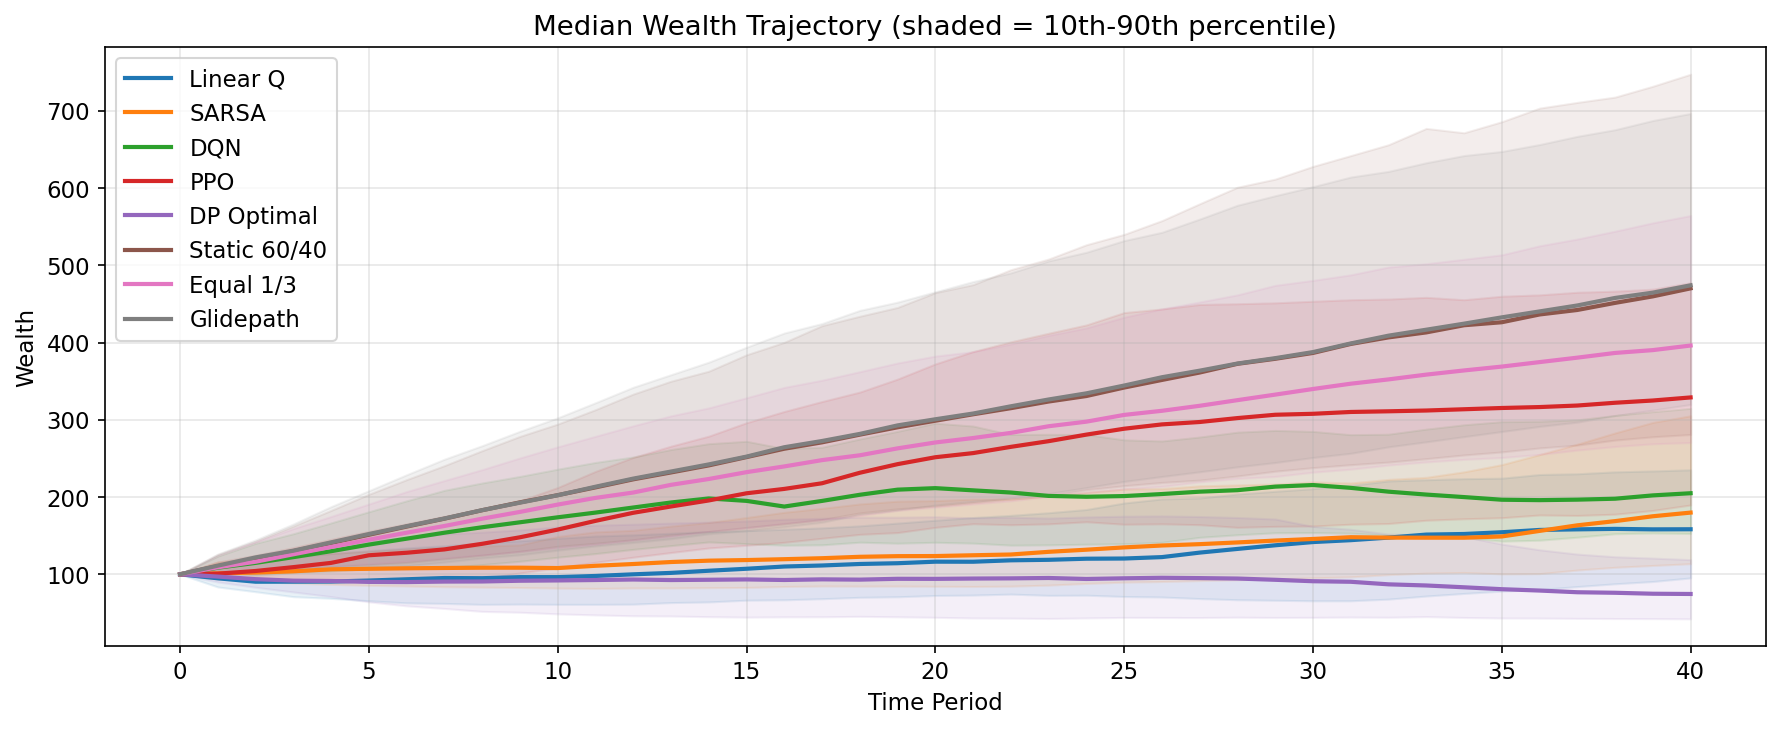
\includegraphics[width=\textwidth]{wealth_trajectories.png}
\end{column}
\begin{column}{0.48\textwidth}
\centering
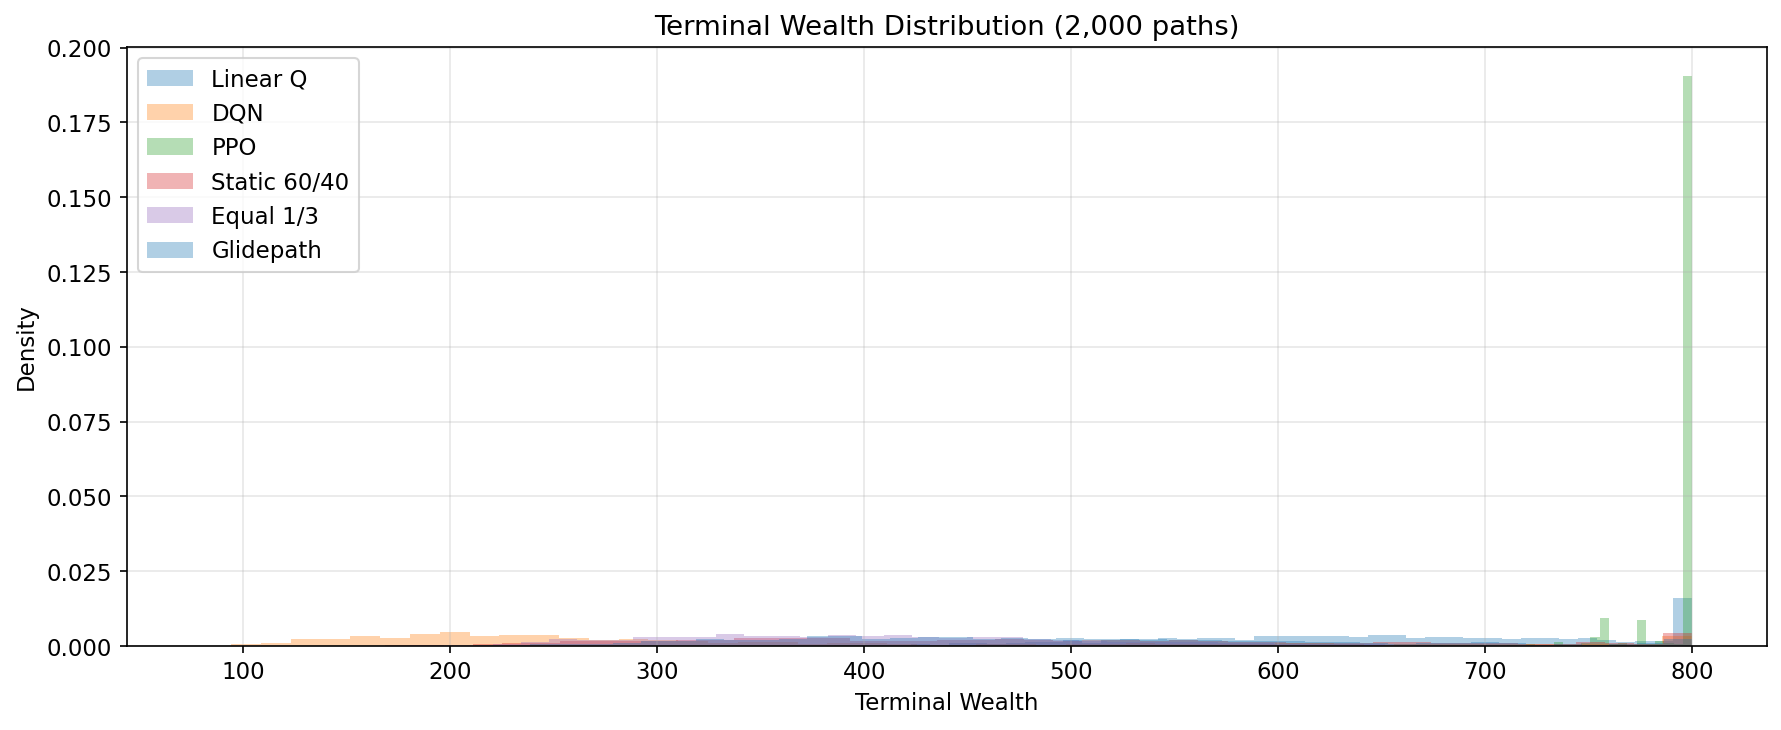
\includegraphics[width=\textwidth]{terminal_wealth.png}
\end{column}
\end{columns}

\vspace{0.5em}
\small
\textbf{Left:} Sample wealth trajectories over 40 years. RL agents (consuming along the way) have lower wealth paths than baselines (which only invest). \textbf{Right:} Terminal wealth distributions. Baselines produce higher but more spread-out terminal wealth; RL agents produce tighter distributions centered on lower values -- by design.
\end{frame}

\note{
\textbf{[Jeffrey speaks -- 45 sec]}\\
``These plots show the story visually. On the left, wealth trajectories: baselines grow to 400-500 because they never consume. RL agents stay around 100-150 because they extract consumption along the way. On the right, terminal wealth distributions: baselines have wide spreads, RL agents have tight, concentrated distributions. The RL agents deliberately traded terminal wealth for lifetime consumption smoothness.''
}

% ============================================================
% SLIDE 21: Utility Distributions
% ============================================================
\begin{frame}{Utility Distributions: RL vs Baselines}
\begin{columns}[T]
\begin{column}{0.58\textwidth}
\centering
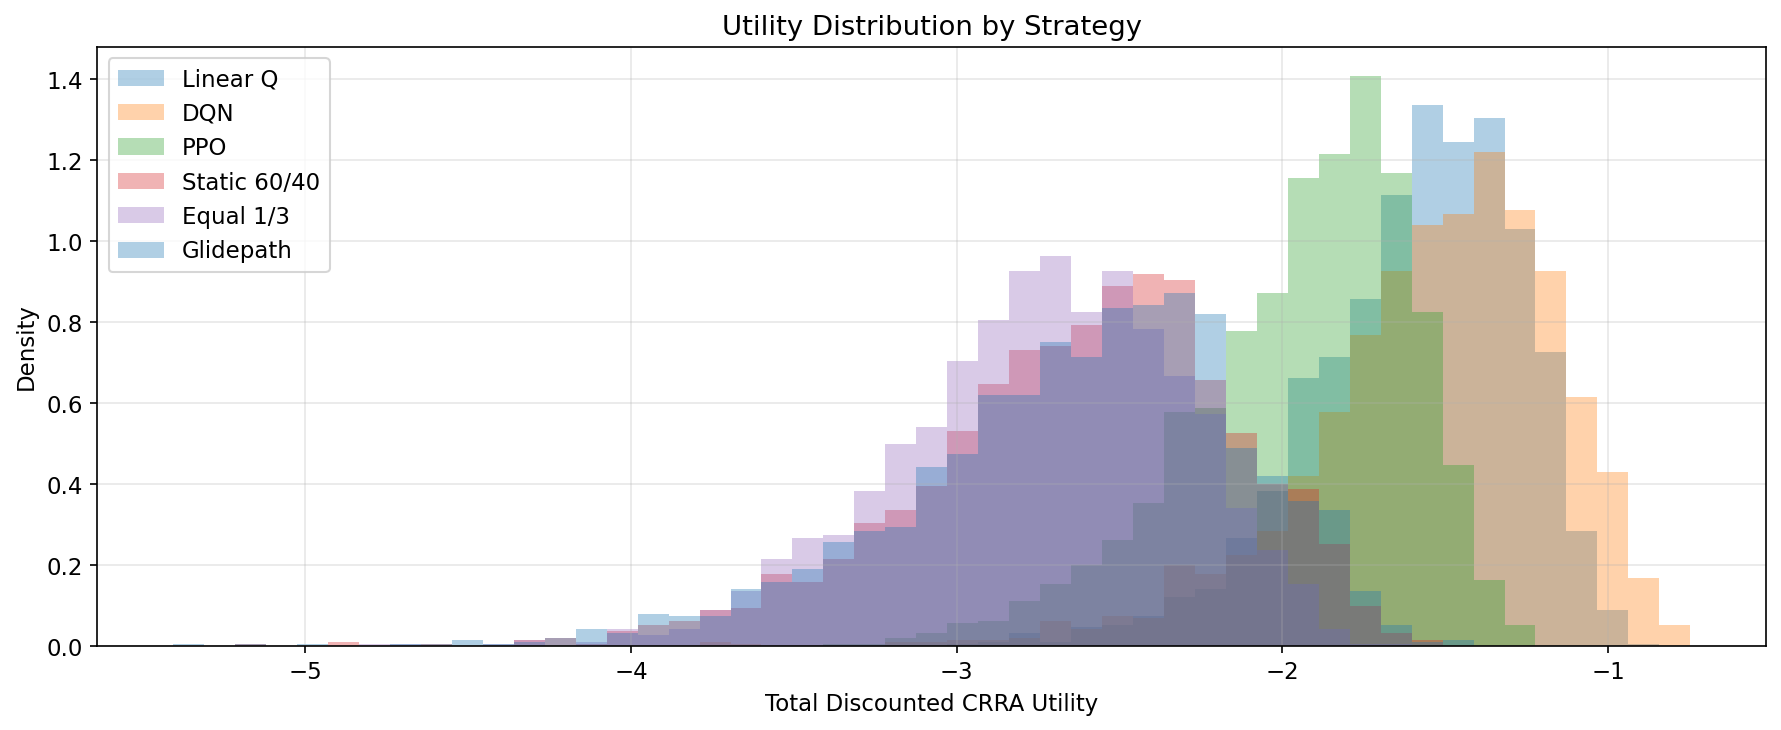
\includegraphics[width=\textwidth]{utility_distributions.png}
\end{column}
\begin{column}{0.40\textwidth}
\textbf{This is the objective.}

\vspace{0.3em}
RL agents (DQN, PPO, Linear Q, SARSA) are shifted \textbf{right} -- higher utility.

\vspace{0.3em}
Baselines (60/40, Equal, Glidepath) cluster left around $-2.5$ to $-3$.

\vspace{0.3em}
\textbf{Key observations:}
\begin{itemize}
    \item DQN has the \textit{tightest} distribution near $-1.5$
    \item Baselines have \textit{long left tails} -- more downside risk in utility space
    \item RL agents' right shift = higher \textit{and} more consistent utility
\end{itemize}
\end{column}
\end{columns}
\end{frame}

\note{
\textbf{[Jeffrey speaks -- 45 sec]}\\
``This histogram is the single most important plot -- it shows the distribution of total discounted CRRA utility across 2,000 simulated lifetimes. Utility is the actual objective we're optimizing.''\\[0.5em]
``The RL agents are clearly shifted to the right -- higher utility. DQN and PPO concentrate tightly near negative 1.5, while baselines spread around negative 2.5 to negative 3 with long left tails. Those left tails are bad outcomes where baselines couldn't adapt to poor market conditions. The RL agents avoid these because they learned state-dependent policies.''
}

% ============================================================
% SLIDE 22: Agent Comparison Summary
% ============================================================
\section{Agent Comparison}

\begin{frame}{Comparing All Four RL Agents}

\begin{center}
\small
\begin{tabular}{lcccc}
\toprule
& \textbf{Linear Q} & \textbf{SARSA} & \textbf{DQN} & \textbf{PPO} \\
\midrule
\textbf{Update target}      & $\max_a Q(s'\!,a)$ & $Q(s'\!, a')$ & $\max_a Q(s'\!,a)$ & Policy gradient \\
\textbf{Function approx}    & Linear (24-dim)    & Linear (24-dim)    & Dueling (256-256) & Sep.\ A-C (256-256) \\
\textbf{Parameters}         & 5,040       & 5,040       & $\sim$122K  & $\sim$191K \\
\textbf{Training time}      & $\sim$18s   & $\sim$15s   & $\sim$23 min & $\sim$2 min \\
\textbf{$\mathbb{E}$[Utility]} & $-1.59$ & $-1.88$     & $\mathbf{-1.54}$ & $-1.95$ \\
\textbf{C-Sharpe}           & 18.30       & 10.25       & \textbf{26.53} & 12.58 \\
\textbf{Min $W_T$}          & \textbf{33.2} & 24.9      & 18.3        & 20.5 \\
\bottomrule
\end{tabular}
\end{center}

\vspace{0.5em}
\textbf{Takeaways:}
\begin{itemize}
    \item \textbf{DQN wins on utility} ($-1.54$) -- Dueling arch + large replay buffer captures nonlinear value
    \item \textbf{Linear agents win on efficiency} -- 5,040 params, trains in seconds, interpretable policy
    \item \textbf{Off-policy $>$ on-policy on utility}: Linear Q beats SARSA; DQN beats PPO
    \item \textbf{All RL agents crush all baselines} -- optimizing the right objective matters most
\end{itemize}
\end{frame}

\note{
\textbf{[Jack speaks -- 1 min]}\\
``Here's the final comparison. The cleanest takeaway: all four RL agents beat all three baselines -- optimizing the right objective matters more than which algorithm you pick.''\\[0.5em]
``Among RL agents, DQN wins on utility at negative 1.54, then Linear Q at negative 1.59. Note the pattern: the off-policy methods (Linear Q, DQN) outperform the on-policy methods (SARSA, PPO). This is consistent with theory -- off-policy methods can bootstrap from the greedy action, learning more aggressively. On-policy methods account for their own exploratory behavior, which makes them more conservative.''\\[0.5em]
``But the linear agents have major practical advantages: 5,040 parameters versus 122K or 191K, trains in 15-18 seconds versus 23 minutes for DQN, and interpretable weights. The utility gap between the best linear agent (Linear Q, -1.59) and the best neural agent (DQN, -1.54) is tiny. For most applications, the linear agents are the pragmatic choice.''\\[0.5em]
``And SARSA specifically: the on-policy update means it doesn't overestimate Q-values from exploratory actions, which is why it's slightly more conservative than Linear Q. In a financial setting, this is arguably desirable -- you don't want a policy that was calibrated assuming future actions are always optimal.''
}

% ============================================================
% SLIDE 22: Conclusions
% ============================================================
\section{Conclusions}

\begin{frame}{Conclusions}

\begin{enumerate}
    \item \textbf{Exact DP works but doesn't scale.}
    Phase 2's backward induction gives the provably optimal solution in 0.4s,
    but a $119\times$ blowup to Phase 3 parameters makes it infeasible.

    \vspace{0.4em}
    \item \textbf{RL handles continuous wealth and richer state spaces.}
    Function approximation replaces the DP table, scaling linearly in episodes
    rather than exponentially in state dimensions.

    \vspace{0.4em}
    \item \textbf{All four RL agents beat all baselines on utility.}
    Off-policy methods (DQN, Linear Q) achieve the best utility; on-policy (SARSA, PPO)
    are simpler and faster. SARSA's on-policy nature gives the most conservative policy.

    \vspace{0.4em}
    \item \textbf{RL optimizes the right objective.}
    Static strategies implicitly optimize wealth. RL directly optimizes \textit{lifetime utility},
    discovering that a risk-averse investor should consume more and invest conservatively
    -- matching financial theory (Merton's solution).
\end{enumerate}

\vspace{0.5em}
\textbf{Future work:} Continuous actions (DDPG/SAC), more assets, transaction costs, real data calibration.
\end{frame}

\note{
\textbf{[Patrick speaks -- 1 min]}\\
``Let me wrap up with four takeaways. First, exact DP gives perfect answers but can't handle realistic problem sizes. Second, RL with function approximation handles the richer problem -- continuous wealth, 3 regimes, 3 income states, 40-year horizon.''\\[0.5em]
``Third, all four RL agents beat all three baselines. The neural network agents get the best raw utility, but the linear agents are dramatically simpler and faster. SARSA in particular produces the most conservative policy thanks to its on-policy update.''\\[0.5em]
``Fourth, and most importantly: RL optimizes the actual objective. Static strategies like 60/40 produce higher wealth, but that's not what a risk-averse investor cares about. The RL agents discovered -- from scratch, through trial and error -- that smooth consumption beats volatile wealth. This is consistent with classical results like Merton's portfolio theory.''\\[0.5em]
``For future work, we'd like to try continuous action spaces using DDPG or SAC, add more asset classes, incorporate transaction costs, and calibrate to real market data.''
}

% ============================================================
% SLIDE 23: Thank You
% ============================================================
\begin{frame}{}
\centering
\vspace{2em}
{\Huge Thank You!}

\vspace{1.5em}
{\Large Questions?}

\vspace{2em}
\normalsize
Repository: \texttt{github.com/yuxiang-jack-zhang/CME241}\\[0.5em]
Relevant textbook sections: Ch.\ 4 (DP), Ch.\ 12.4 (SARSA), Ch.\ 12.6 (Q-Learning), Ch.\ 13 (Policy Gradient)
\end{frame}

\note{
\textbf{[All -- open for questions]}\\
\textbf{Likely questions and answers:}\\[0.3em]
\textit{``Why does RL have lower wealth but better utility?''} -- Because CRRA utility with gamma=2 is extremely risk-averse. Marginal utility of consumption diminishes fast, so smooth consumption over 40 years beats a large volatile nest egg. The math: u(c) = -1/c, so doubling consumption from 10 to 20 gives more utility gain than going from 100 to 110.\\[0.3em]
\textit{``Why is gamma=1 in the TD update if beta=0.96?''} -- Because beta is already baked into the rewards as beta\^{}t * u(c\_t). Using gamma=0.96 in the update would double-discount. gamma=1 with discounted rewards correctly recovers the CRRA objective.\\[0.3em]
\textit{``Why does DQN beat SARSA?''} -- DQN is off-policy: it uses max Q(s',a) in its target, learning from the optimal greedy policy regardless of exploration. SARSA uses Q(s', a') where a' is the exploratory action actually taken, which is more conservative. In this problem, the equity premium is strong enough that the aggressive off-policy updates pay off.\\[0.3em]
\textit{``Why not use eligibility traces (SARSA($\lambda$))?''} -- With 40-step episodes, TD(0) already propagates value well. Adding traces could help early in training but adds hyperparameter complexity. Future work.\\[0.3em]
\textit{``Is SARSA convergence guaranteed here?''} -- Not with function approximation. Theorem 12.4.1 is for tabular. But linear FA + on-policy is the safest combination -- avoids the deadly triad of FA + bootstrapping + off-policy.\\[0.3em]
\textit{``How does Phase 3 DP compare?''} -- We ran the DP solver on the Phase 3 environment (discretized wealth). It achieves E[Utility] = -1.456, confirming RL agents are close to optimal. DQN at -1.54 is only a 5\% optimality gap.\\[0.3em]
\textit{``What's the deadly triad?''} -- Function approximation + bootstrapping + off-policy learning. This combination can cause Q-value divergence. SARSA avoids it (on-policy). DQN works around it with target network + replay buffer.
}

\end{document}
